\documentclass[letterpaper]{report}

\usepackage{calc,amsmath,amssymb,amsfonts}
\usepackage[T1]{fontenc}
\usepackage[english]{babel}
\usepackage{xcolor}
\usepackage[top=2cm,bottom=1.27cm,left=3cm,right=2cm,includefoot]{geometry}
\usepackage[style=numeric,backend=biber]{biblatex}
\usepackage{array,supertabular,hhline,hyperref}
\usepackage[pdftex]{graphicx}
\usepackage[final]{pdfpages}
\usepackage{tabularx}

% this package best loaded last in the preamble
\usepackage{subfiles} 

\hypersetup{colorlinks=true,allcolors=blue,pdftitle=Screen Specification,pdfauthor=Bui Hoang Tu 20200547}
\setlength\tabcolsep{1mm}
\renewcommand\arraystretch{1.3}
\title{AIMS Screen Specification}
\author{Bui Hoang Tu 20200547}
\date{2023-10-15}

%%%%%%%%%%%%%%%%%%%%%%%%%%%%%%%%%%%%%%%%%%%%%%%%%%%%%%%%%%%%%%%%%%%%%%%%%%%%%%%%%
\begin{document}
    \textbf{View cart screen}
    \begin{itemize}
        \item \textbf{Date of creation}: ??
        \item \textbf{Approved by}: ??
        \item \textbf{Reviewed by}: ??
        \item \textbf{Person in charge}: ??
    \end{itemize}

    \begin{center}
        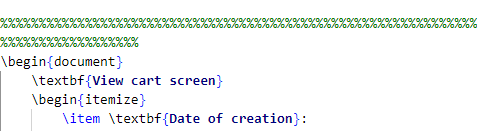
\includegraphics[width=0.8\textwidth]{ScreenHolder.png}
    \end{center}

    \begin{tabular*}{0.9\linewidth}{|c|c|c|}
        \hline
        \textbf{Control} &
        \textbf{Operation} &
        \textbf{Function} \\
        \hline

        Area for displaying the subtotal &
        Initial &
        Display the subtotal \\
        \hline

    \end{tabular*}
\end{document}